% !TEX pdflua

%%%%%%%%%%%%%%%%%%%%%%%%%%%%%%%%%%%%%%%%%
% Wilson Resume/CV
% XeLaTeX Template
% Version 1.0 (22/1/2015)
%
% This template has been downloaded from:
% http://www.LaTeXTemplates.com
%
% Original author:
% Howard Wilson (https://github.com/watsonbox/cv_template_2004) with
% extensive modifications by Vel (vel@latextemplates.com)
%
% License:
% CC BY-NC-SA 3.0 (http://creativecommons.org/licenses/by-nc-sa/3.0/)
%
%%%%%%%%%%%%%%%%%%%%%%%%%%%%%%%%%%%%%%%%%

%----------------------------------------------------------------------------------------
%	PACKAGES AND OTHER DOCUMENT CONFIGURATIONS
%----------------------------------------------------------------------------------------
\documentclass[10pt]{article} % Default font size

%%%%%%%%%%%%%%%%%%%%%%%%%%%%%%%%%%%%%%%%%
% Wilson Resume/CV
% Structure Specification File
% Version 1.0 (22/1/2015)
%
% This file has been downloaded from:
% http://www.LaTeXTemplates.com
%
% License:
% CC BY-NC-SA 3.0 (http://creativecommons.org/licenses/by-nc-sa/3.0/)
%
%%%%%%%%%%%%%%%%%%%%%%%%%%%%%%%%%%%%%%%%%

%----------------------------------------------------------------------------------------
%	PACKAGES AND OTHER DOCUMENT CONFIGURATIONS
%----------------------------------------------------------------------------------------

\usepackage[a4paper, hmargin=25mm, vmargin=30mm, top=20mm]{geometry} % Use A4 paper and set margins

\usepackage{fancyhdr} % Customize the header and footer

\usepackage{lastpage} % Required for calculating the number of pages in the document

\usepackage{hyperref} % Colors for links, text and headings

\setcounter{secnumdepth}{0} % Suppress section numbering

%\usepackage[proportional,scaled=1.064]{erewhon} % Use the Erewhon font
%\usepackage[erewhon,vvarbb,bigdelims]{newtxmath} % Use the Erewhon font
\usepackage[utf8]{inputenc} % Required for inputting international characters
\usepackage[T1]{fontenc} % Output font encoding for international characters

\usepackage{fontspec} % Required for specification of custom fonts
\setmainfont[Path = ./fonts/,
Extension = .otf,
BoldFont = Erewhon-Bold,
ItalicFont = Erewhon-Italic,
BoldItalicFont = Erewhon-BoldItalic,
SmallCapsFeatures = {Letters = SmallCaps}
]{Erewhon-Regular}

\usepackage{color} % Required for custom colors
\definecolor{slateblue}{rgb}{0.17,0.22,0.34}

\usepackage{sectsty} % Allows customization of titles
\sectionfont{\color{slateblue}} % Color section titles

\fancypagestyle{plain}{\fancyhf{}\cfoot{\thepage\ of \pageref{LastPage}}} % Define a custom page style
\pagestyle{plain} % Use the custom page style through the document
\renewcommand{\headrulewidth}{0pt} % Disable the default header rule
\renewcommand{\footrulewidth}{0pt} % Disable the default footer rule

\setlength\parindent{0pt} % Stop paragraph indentation

% Non-indenting itemize
\newenvironment{itemize-noindent}
{\setlength{\leftmargini}{0em}\begin{itemize}}
{\end{itemize}}

% Text width for tabbing environments
\newlength{\smallertextwidth}
\setlength{\smallertextwidth}{\textwidth}
\addtolength{\smallertextwidth}{-2cm}

\newcommand{\sqbullet}{~\vrule height 1ex width .8ex depth -.2ex} % Custom square bullet point definition

%----------------------------------------------------------------------------------------
%	MAIN HEADER COMMAND
%----------------------------------------------------------------------------------------

\renewcommand{\title}[1]{
{\huge{\color{slateblue}\textbf{#1}}}\\ % Header section name and color
\rule{\textwidth}{0.5mm}\\ % Rule under the header
}

%----------------------------------------------------------------------------------------
%	JOB COMMAND
%----------------------------------------------------------------------------------------

\newcommand{\job}[6]{
\begin{tabbing}
\hspace{2cm} \= \kill
\textbf{#1} \> \href{#4}{#3} \\
\textbf{#2} \>\+ \textit{#5} \\
\begin{minipage}{\smallertextwidth}
\vspace{1mm}
#6
\end{minipage}
\end{tabbing}
\vspace{1mm}
}

%----------------------------------------------------------------------------------------
%	SKILL GROUP COMMAND
%----------------------------------------------------------------------------------------

\newcommand{\skillgroup}[2]{
\begin{tabbing}
\hspace{5mm} \= \kill
\sqbullet \>\+ \textbf{#1} \\
\begin{minipage}{\smallertextwidth}
\vspace{2mm}
#2
\end{minipage}
\end{tabbing}
}

%----------------------------------------------------------------------------------------
%	INTERESTS GROUP COMMAND
%-----------------------------------------------------------------------------------------

\newcommand{\interestsgroup}[1]{
\begin{tabbing}
\hspace{5mm} \= \kill
#1
\end{tabbing}
\vspace{-10mm}
}

\newcommand{\interest}[1]{\sqbullet \> \textbf{#1}\\[3pt]} % Define a custom command for individual interests

%----------------------------------------------------------------------------------------
%	TABBED BLOCK COMMAND
%----------------------------------------------------------------------------------------

\newcommand{\tabbedblock}[1]{
\begin{tabbing}
\hspace{2cm} \= \hspace{4cm} \= \kill
#1
\end{tabbing}
}

\newcommand{\jobtechnologies}[1]{
\rule{0mm}{5mm}\textbf{Technologies:} #1   
}

\newcommand{\opensource}[2]{
\tabbedblock{
\bf{#1} \> #2
}
}
 % Include the file specifying document layout
\usepackage{fontawesome}
\usepackage{xcolor}
\usepackage{graphicx}
\hypersetup{
    colorlinks,
    linkcolor={red!50!black},
    citecolor={blue!50!black},
    urlcolor={blue!80!black}
}
\usepackage{array}
\usepackage{worldflags}


%----------------------------------------------------------------------------------------

\begin{document}

%----------------------------------------------------------------------------------------
%	NAME AND CONTACT INFORMATION
%----------------------------------------------------------------------------------------

    \title{Tomáš Heřman} % Print the main header

%------------------------------------------------

    \parbox{0.5\textwidth}{ % First block
        \begin{tabular}{ m{0.1em} m{5.5em} m{12em} } % Enables tabbing
            \faicon{map}           & \textbf{Address}     & Zurich,                                                       \\
            &                      & Switzerland                                                \\% Address line 2
            \faicon{birthday-cake} & \textbf{Birthday}    & 21$^{st}$ February 1989                                       \\ % Date of birth
            \faicon{flag}          & \textbf{Nationality} & Czech                                                         \\ % Nationality
            \faicon{phone}         & \textbf{Phone}       & +420 728 466 416                                              \\ % Mobile phone
            &                      & +410 778 09 51 34                                             \\ % Mobile phone
            \faicon{envelope}      & \textbf{Email}       & \href{mailto:tomas.herman@gmail.com}{tomas.herman@gmail.com}  \\ % Email address
            \faicon{github}        & \textbf{GitHub}      & \href{https://github.com/tomasherman}{github.com/tomasherman} \\
            \faicon{language}      & \textbf{Languages}   & Czech: \textit{Native}                                        \\
            &                      & English: \textit{Fluent}

        \end{tabular}}
    \hfill % Horizontal space between the two blocks
    \parbox{0.5\textwidth}{ % Second block
        \begin{tabbing} % Enables tabbing
            \hspace{3cm} \= \hspace{4cm} \= \kill % Spacing within the block
            \fbox{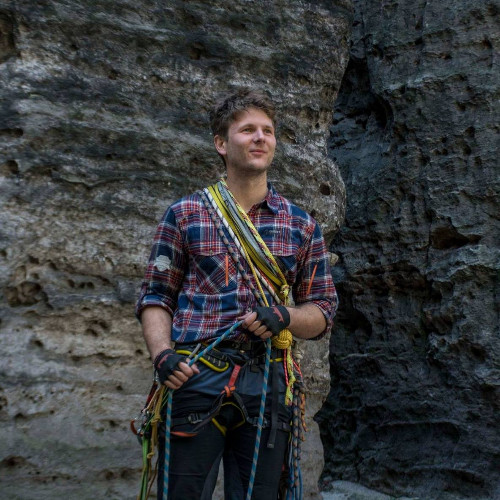
\includegraphics[height=4cm]{photo.jpeg}} \\
        \end{tabbing}}

%----------------------------------------------------------------------------------------
%	PERSONAL PROFILE
%----------------------------------------------------------------------------------------


    \section{Open source}
    \opensource{\href{https://github.com/avast/datadog4s}{datadog4s}}{Monitoring library for Cats-Effect based scala application.}

%----------------------------------------------------------------------------------------
%	EMPLOYMENT HISTORY SECTION
%----------------------------------------------------------------------------------------


    \section{Employment History}

    \job
    {Aug 2021 -}{Present}
    {Avast Software, Prague \& Zurich}
    {http://www.avast.com}
    {Senior Software/Data engineer}
    {After \href{https://www.avast.com/en-us/omni}{Omni project} was cancelled and my team dissolved, I joined a Big Data team. I was tasked with making various improvements
    to many of the existing components of the big data solution. Most notably, I participated on migration and modernisation of on-prem big data solution to GCP. In addition to programming and redesigning of old services, this included a lot of Ops work as well (setup of terraform, GKE, monitoring \& alerting).\\

    \jobtechnologies{Scala, Java, Kafka, Kubernetes, GCP, Terraform}}


    \job
    {Aug 2019-}{Aug 2021}
    {Avast Software, Prague}
    {http://www.avast.com}
    {Team Lead, Senior Software engineer}
    {Promoted to lead a team of 3 (and later 6) backend-developers at \href{https://www.avast.com/en-us/omni}{Omni project}. In addition to Team Lead duties (1 on 1s, Sprint plannings, hiring (for my and other teams)), I also spent a lot of time talking to Product about new features, improvements and ideas. I helped design said features and make sure they get implemented on time and in adequate quality. I took care about making sure that estimates are realistic and what we commit to is feasible and relevant. \\

    \jobtechnologies{Scala, Cassandra, Kafka, RabbitMQ, Netty, Http4s, cats-effect, Netty, Kubernetes, Helm, AWS, Terraform}}

%------------------------------------------------

    \job
    {Mar 2016 -}{Aug 2019}
    {Avast Software, Prague}
    {http://www.avast.com}
    {Software Engineer}
    {I worked on various services related to Avast AntiVirus and other supporting systems. In addition to coding,
        I played a big role in introducing (Scala) Functional Programming to other engineers. I (with few others) prepared many talks, libraries, workshops etc. \\ Some interesting projects I worked on:
        \begin{itemize}
            \item DNS proxy written in Netty \& Scala
            \item System for scanning Android APKs for Avast partners
            \item High throughput, highly cost-sensitive websocket server for \href{https://www.avast.com/en-us/omni}{Avast Omni} project
        \end{itemize}

        \jobtechnologies{See Above}}

%------------------------------------------------

    \job
    {2014 -}{Feb 2016}
    {Golem Trading for Wikidi, Prague, Czech Republic}
    {https://www.golemtrader.com/}
    {Software engineer}
    {I returned to Wikidi to work in a very small team on Golem trading platform. I worked on \emph{Trader} app which made decision about trading and I also wrote an UI for the founder/thought leader to watch/control what the trader is doing. Eventually, I became the lead for the platform. \\
    \jobtechnologies{Java, Kotlin, \href{https://en.wikipedia.org/wiki/Financial_Information_eXchange}{FIX}, ReactJS, Google Sheets updated via Python}}

%------------------------------------------------

    \job
    {2013 -}{2014 }
    {Spinoco, Prague, Czech Republic}
    {https://www.spinoco.com/}
    {Solution Designer}
    {Worked as a full-stack (but mostly back-end) developer in a small team on a Telco app, which used very advanced Scala concepts/tools like scalaz-streams or ScalaJS. In addition to developer work I also had a chance to interact with clients and even attended a sales meeting.\\
    \jobtechnologies{Scala(JS), Scalaz Streams (later evolved into FS2 streams), Scalaz, Play Framework, Cassandra}}

%------------------------------------------------

    \job
    {2012 -}{2013}
    {Magic Table project for Wikidi, Prague, Czech Republic}
    {https://www.magictable.com}
    {Developer}
    {I was the sole developer on the project (lead by \href{https://michal.illich.cz/}{the founder}). I was responsible for web-crawling, data processing pipeline, applying machine learning libraries and basically everything else. \\
    \jobtechnologies{Python, R}}

%------------------------------------------------

%----------------------------------------------------------------------------------------
%	EDUCATION SECTION
%----------------------------------------------------------------------------------------


    \section{Education}

    \tabbedblock{
        \bf{2008-2012} \> BCs. in Intelligent Systems - \href{https://www.cvut.cz/}{Czech Technical University, Prague} \\[5pt]
        \> As a final project I wrote MineCraft server in Scala and Akka
    }

%----------------------------------------------------------------------------------------
%	IT/COMPUTING SKILLS SECTION
%----------------------------------------------------------------------------------------


    \section{Software Engineering Skills}

    \skillgroup{Programming Languages}
    {
        \textit{Scala} - Lot of experience with Typelevel stack (http4s, cats-effect, etc), weapon of choice\\
    \textit{Java} - Used in past and at University\\
    \textit{Python} - Used in past and for ad-hoc scripts etc.\\
    }

%------------------------------------------------

    \skillgroup{Operations and Cloud}
    {
        \textit{Kubernetes, Helm} - maintenance and development of helm/kubernetes services\\
        \textit{AWS, GCP, Terraform, Spinnaker} - as a user, not as administrator \\
    \textit{Grafana, Datadog, Icinga, VictorOps} - as a user, not as administrator \\
    }

    \skillgroup{Others}
    {
        \textit{Git, Bash} \\
        \textit{Cassandra, Kafka, RabbitMQ, SQL Databases}
    }


%----------------------------------------------------------------------------------------
%	INTERESTS SECTION
%----------------------------------------------------------------------------------------


    \section{Interests}

    \interestsgroup{
        \interest{Running, hiking, weight-lifting}
        \interest{(Teaching) Rock climbing - 5+ years of teaching experience as an instructor}
        \interest{Investing and finance}
    }


%----------------------------------------------------------------------------------------
%	OTHER SECTION
%----------------------------------------------------------------------------------------



%----------------------------------------------------------------------------------------
%	REFEREE SECTION
%----------------------------------------------------------------------------------------

% \section{Referees}
%
% \parbox{0.5\textwidth}{ % First block
% \begin{tabbing}
% \hspace{2.75cm} \= \hspace{4cm} \= \kill % Spacing within the block
% {\bf Name} \> Bill Lumbergh \\ % Referee name
% {\bf Company} \> Initech Inc. \\ % Referee company
% {\bf Position} \> Vice President \\ % Referee job title
% {\bf Contact} \> \href{mailto:bill@initech.com}{bill@initech.com} % Referee contact information
% \end{tabbing}}
% \hfill % Horizontal space between the two blocks
% \parbox{0.5\textwidth}{ % Second block
% \begin{tabbing}
% \hspace{2.75cm} \= \hspace{4cm} \= \kill % Spacing within the block
% {\bf Name} \> Michael "Big Mike" Tucker\\ % Referee name
% {\bf Company} \> Burbank Buy More \\ % Referee company
% {\bf Position} \> Store Manager \\ % Referee job title
% {\bf Contact} \> \href{mailto:mike@buymore.com}{mike@buymore.com} % Referee contact information
% \end{tabbing}}
%
% %----------------------------------------------------------------------------------------
%
\end{document}
